
%%%%%%%%%%%%%%%%%%%%% Introduction %%%%%%%%%%%%%%%%%%%%%%%%%%%%%%%%%

\section{Introduction}

\subsection{Aim of the study}
Chronic lymphatic leukemia is a heterogeneous disease characterized by phenotypic and genotypic variety, which indicates specific regulation on molecular level. Optimal treatment of such a complex disease needs personalized medicine with individually adapted therapeutic interventions. Personalized medicine relies on understanding the pathogenic molecular mechanisms and defining genotype marker for them. This study aims to characterize the most common genotypes and underlying mechanistic changes of chronic lymphatic leukemia by gene expression analysis. Enrichment analysis and differential expression analysis of RNA sequencing data are used to define gene signatures typical for common variants. Thereby, integration of data from methylome analysis, drug response assays, FISH analysis and clinical metadata provide a basis to study and interpret gene expression changes in depth.  


\subsection{Chronic lymphatic leukemia}
Chronic lymphatic leukemia (CLL) is defined as an accumulation of $CD23^{+}CD19^{+}CD5^{+}$ mature clonal B lymphcytes with $>5000$ cells/ml blood. With an incidence of $4.5/100,000$ people per year it is the most abundant form of adult leukemia \citep{Fabbri2016}. CLL is usually characterized by an initially slow growth and late development with a median age of diagnosis of 70 years. Other than this, the course of disease and clinical outcome vary a lot. Some patients develop a slow growing form with good response to chemotherapeutics and only slight decrease in life expectancy. Other patients show an aggressive type with fast tumor growth, resistance to chemotherapeutics and poor prognosis. Large cohort studies using next generation sequencing technologies unraveled a highly variable genotypic and epigenetic landscape behind prototypic heterogeneity. Furthermore, targeted therapeutics have been developed and are further investigated. Thus, the identification of mechanisms behind phenotypic and genotypic variability in CLL is a great chance for a next step forward in perzonalized medicine \citep{Guieze2015}.      


\subsubsection{Common genetic variants}
CLL is characterized by a genetic and phenotypic heterogeneity. Despite the fact that it has been studied intensively, no explicit driving genotype has been identified, but a landscape of genetic alterations in interaction with microenvironmental factors seems to define the tumor \citep{Rossi2016}. In total more than 2000 molecular changes have been associated with the CLL genome including copy number variations (CNVs), insertions and deletions (InDels) and functional mutations \citep{Puente2015}. Often, those changes occur at low frequencies and or in combination. Advances in sequencing technologies enabled whole-exome sequencing (WES) of large cohorts resulting in a set of 55 major mutations and CNVs \citep{Landau2015}. The following most frequent genetic variants are analyzed in this study.

\paragraph{IGHV status}
Two subtypes of CLL can be classified by occurrence of somatic hypermutation in the Ig heavy-chain variable region. The IGHV-unmutated group has $\geq 98\%$ homology with the germline sequence of the IGHV gene locus, whereas the IGHV-mutated group is characterized by hypermutations and $< 98\%$ IGHV germline identity \citep{Burns2017}. Groups differ significantly in clinical outcome and therapeutic response with better prognosis and overall survival in the IGHV-mutated group. IGHV mutation status is related to antigen binding and activation of B cell receptor (BCR) signaling. Subtypes derive from different stages of maturated B-cells, which have been exposed to different receptor stimulation processes. In IGHV-unmutated cells, the BCR shows low-affinity and is poly- or self-reactive, whereas IGHV-mutated cells express mono or oligo-reactive BCRs \citep{Fabbri2016}. On expression level, tyrosine kinase Zap70 works as a marker that correlates with BCR signaling and is overexpressed in IGHV unmutated cells \citep{Stevenson2011}. A second indicative marker is CD38, which regulates cell activity, proliferation and adhesion \citep{Cruse2007}.   


\paragraph{Trisomy12}
With an incidence of 15\% Trisomy12 is among the most common chromosomal aberrations in CLL. It is associated with an increased risk to develop secondary tumors and poor outcome in combination with Notch1 mutations \citep{Fabbri2016}. Despite the prognostic changes, Trisomy12 has not been distinctly associated to pathway activity changes on molecular level. One study found increased expression of surface integrins like CD11b (ITGAM), CD18 (ITGB2), CD29 (ITGB1) and ITGB7 and intracellular integrin signaling molecules like RABP-1. These changes are related to the very late antigen-4 (VLA-4) directed leukocyte adhesion cascade, which regulates migration into the pro-survival environment of the lymphnode \citep{Riches2014}. VLA-4 is an integrin dimer of CD29 (ITGB2) and CD49D(ITGA4).

\paragraph{Del13q14}
With an incidence of $>60$\%, deletion of the 13q14 locus is the most frequent genetic variation in CLL. The length of deletion differs among patients, but all span the region of the long non-coding RNAs DLEU2 and DLEU1, the microRNAs MIR15A-MIR16-1 and the gene DLEU7. The role of these transcripts in tumor developement as well as underlying mechanisms is not completely understood yet. MicroRNA complex miR15A-miR16-1 plays a role in cell cycle arrest and the regulation of apoptosis resistance gene BCL-2. How this is related to DLEU deletion and other genetic lesions remains to be investigated \citep{Aqeilan2009}.
 
\paragraph{TP53 and Del17p13} 
Tumor suppressor gene TP53 resides on chromosome band 17p13. TP53 is an important regulator of DNA damage control and its homozygotic inactivation is a common feature of many tumors. CLL patients with Del17p13 often ($\sim80\%$) have an inactivating mutation in the remaining TP53 gene. Some patients also develop TP53 mutations in both allels \citep{Fabbri2016}. The role of heterogenetic inactivated TP53, either by deletion or mutation is not clear. There could be another way of inactivation of the remaining allel or it could be a secondary event developed during the course of tumor.

\paragraph{Del11q22 and ATM}
ATM is another regulator of DNA damage response. Thus, CLLs with ATM mutations are characterized by genomic instability. It is located in the region of Del11q22 and in patients with ATM mutation and Del11q22 homozygotic inactivated. The role of heterogenetic ATM inactivation needs to be further elucidated. Del11q22 also span BIRC3, which is a regulator of NF-kB pathway. In total about 20\% of CLL patients show a Del11q22 genotype \citep{Fabbri2016}.  

\paragraph{Notch1}
Notch1 gene encodes a transmembrane receptor. In CLL patients, the activating Notch1 mutation results in up regulation of ligand-dependent pathway genes like RBPJ, MAML1 and ICN1. Other genetic lesions, such as Trisomy12 and IGHV-mutation, are also associated with a deregulated Notch1 pathway. In line with this, patients with Notch1 mutation vary in their clinical features and prognosis depending on their further genotype \citep{Fabbri2016}.  

\paragraph{SF3B1}
As part of the spliceosome, SF3B1 mutations cause aberrant splicing patterns in CLL patients. How these differences in RNA processing are reflected on gene expression levels and their function in tumor progression are unknown. SF3B1 mutations are often associated with Del11q22, suggesting promotive functions. Furthermore, mutations have also been found in other regulators of RNA processing, which suggests an important role of the spliceosome machinery in CLL. SF3B1 mutated CLLs are associated with poor prognosis \citep{Fabbri2016}.

\paragraph{Del8p12 and Gain8q24}
Genomic rearrangements at chromosome 8 are part of the genomic landscape of CLL. The locus 8q24 includes the MYC gene and is associated with aggressive tumor progession. Gain8q24 is often downstream of other mutations and found in complex karyotypes \citep{Li2016}. Deletions at 8p12 show a wide range in the size of the deleted DNA sequence and have been associated to a short time to first treatment. Mechanistic changes underlying these variants are unknown yet \citep{Brown2012}. 


\paragraph{BRAF}
BRAF mutations are common in different cancer types and occur at low frequencies in CLL patients. It has been difficult to associate BRAF mutations to a distinct CLL phenotype \citep{Jebaraj2013}. However, in a case study BRAF inhibitor induced activation of ERK and caused CLL progression, suggesting a possible relation to the MEK/ERK pathway in BRAF mutated CLL patients \citep{Jebaraj2013}.  


\paragraph{MED12}
MED12 is part of the Mediator protein complex. Mediator is a transcription activation regulator and its dysregulation is associated with the development of several severe diseases. In CLL different mutations in MED12 are known. They are associated with loss of Mediator-associated CDK kinase activity. MED12 mutations are correlated with IGHV-unmutated status and poor prognosis \citep{Kampjarvi2015}.  


\paragraph{Methylation status}
Epigenome analysis revealed differences in methylation pattern within CLL patients. They can be divided into 3 subtypes: High-, Intermediate- and Low-programmed (HP, IP and LP), which differ in the amount of hyper-methylated sites. These groups reflect methylation states of memory B-cells during maturation. As CLL tumor cells show a high degree of clonality in methylation pattern, differences could be inherited from the tumor originating cell reflecting its state of maturation \citep{Oakes2016}. This is in line with a correlation of LP subtypes and IGHV-unmutated group and HP subtype and IGHV-mutated group. IGHV groups represent B cells from different stages in the maturation process. Tumor associated differences in methylation groups were found in transcription factor dysregulation of EGR, NFAT, EBF and AP1.


\subsection{The primary blood cancer cell encyclopedia}
This study focuses on transcriptome data from the Primary Blood Cancer Cell Encyclopedia (PACE) \citep{Dietrich}. PACE is a collaborative effort of the National Center of Tumor diseases (NCT) Heidelberg, the German Cancer research Center (DKFZ) Heidelberg and the European Molecular Biology Laboratory (Embl) Heidelberg. It provides a multiomics data collection for the same cohort of patients, including 249 leukemia patients with 184 cases of chronic lymphocytic leukemia (CLL). Major datasets can be split into 4 categories: Geneotype data, transcriptome data, methylome data and drug response data. Geneotype data include gene mutations, single nucleotide polymorphisms (SNPs) and copy number variations (CNVs) and were generated by Whole Genome Sequencing (WGS), Whole Exome Sequencing (WES), SNP arrays and Fluorescence in sito hybridization (FISH). Transcriptome data were generated using bulk RNA sequencing. Genome-wide DNA methylation profiles were derived from DNA methylation arrays. Drug sensitivities of 63 compounds at five concentrations were measured using ATP-based viability assays. Besides this, clinical data, metabolic data and patient metadata are available. A prior multi-variable study investigated the PACE datasets in order to understand the heterogeneous drug response pattern in CLL patients, and stratify patient into different drug response groups\citep{Dietrich}.


\subsection{Transcriptome analysis}
The transcriptome represents the sum of expressed genes in a cell. It includes protein coding messenger RNA, as well as regulatory transcripts like non-coding RNA and small RNA. Transcriptomic profiling aims to describe RNA type, structure and quantity in a certain cell type under specific conditions.
Nowadays, the standard tool for gene expression analysis is RNA sequencing (RNA-seq). RNA-seq is a high throughput next-generation sequencing (NGS) technology. Basically, RNA is extracted from a cell population or single cells, fragmented and converted into a cDNA library. Library molecules are flagged with adapters, which serve as sequencing start sides and sample identifier. Afterwards all reads are amplified and sequenced from both sides (paired-end) or one side (single-end) using NGS. Resulting sequences are computationally analyzed \citep{Wang2009}.  

\subsubsection{Preprocessing}
First steps of RNA-seq analysis include quality control and read filtering. Nucleotide content, base call precision and overrepresented sequences are examined. Reads, that contain adapter sequences, are trimmed and if the base call precision remarkably drops towards the end of reads, quality trimming can be performed.    

\subsubsection{Alignment}
To determine type and quantity of sequenced RNA, reads need to be annotated towards the gene or transcript they originate from. Different methods exist to either map reads to a reference genome or a transcript assembly. Spliced Transcripts Alignment to a Reference (STAR) is a common tool to align RNA-reads from non-contiguous spliced transcripts directly against a reference genome. Thereby STAR basically uses a two step algorithm. First, during the seed search step STAR looks for Maximal Mappable Prefixes (MMPs). MMPs are the longest substrings in a read, which exactly map against the reference genome. For unmapped parts of the read STAR searches independently in a second run. This enables the detection of splice junction without a priori information and increases the mapping speed. Second, STAR generates one alignment for the entire read, by clustering all seeds together and 'stitching' them to one alignment allowing for multiple mis-mappings, but only one insertion or deletion. A local alignment scoring scheme is used to define the best alignment \citep{Dobin2015}.
For transcript quantification aligned reads are summarized into read counts. Thereby the number of read fragments overlapping with a gene is determined. A gene is defined by the sum of related  exons and provided as gene model in Genome Transfer Format (GTF) \citep{Anders2010}.


\subsubsection{Exploratory Data Analysis and Quality control}
Exploratory data analysis (EDA) aims to give a general overview of the data and its structure. It serves as a quality control and can identify technical or experimental issues, such as batch effects, but also give important insight into the data. Methods to investigate sample relationships are principal component analysis (PCA), sample and gene clustering. This ensures data quality and suitability to answer the study's main questions, but also serves to identify confounding factors and major trends of gene expression. 

\paragraph{Variance stabilizing transformation}
Usually raw gene expression data (RNA-Seq counts) show higher variance with a higher mean. However, many statistical tests and regression models (for example, least sum of squares) rely on all data having about the same variance. A remedy is variance stabilizing transformation (VST). Common examples are the logarithmic transformation for data with a constant coefficient of variation ($\text{sd}\propto\text{mean}$) and the square root transformation for data with a Poisson distribution, where $\text{var}\propto\text{mean}$. After transformation, the data will have similar variances across the dynamic range, i.\,e., across different mean values. However, for RNA-Seq data, the mean-variance is more complex than either of these simple examples; in fact, it is a combination of both. A VST can still be found \citep{Anders2010}. It turns out to be a monotonic function that is similar to $f(x)=\sqrt(x)$ for small values of $x$, to $f(x)=\log_2(x)$ for high values of $x$, and a smooth interpolation in between.

Note: It is important to note that \emph{variance} in this context refers to the variance between repeated measurements of the same underlying, true quantity, i.\,e., between replicates -- not, variance of a set of measurements of different underlying true values, e.\,g., between different treatments or disease groups.

\subsubsection{Differential gene expression}
To identify differentially expressed genes between different conditions, cell types or in this case genetic variants is a major application of RNA-seq analysis. It aims to unravel molecular mechanisms behind phenotypic variation. A common tool for comparative transcriptome analysis is DESeq2. DESeq2 tests for differences in the logarithmic fold changes (LFC) of gene expression between two groups or conditions. For each gene it calculates generalized linear models (GLMs) to determine gene dispersion and size factors within the different groups. Size factors are fitted as normalized numbers of fragments mapping to each gene. Read counts are modeled as a negative binomial distribution. For different conditions the within-group variability is estimated by a dispersion parameter. Thereby, genes with a similar average expression are assumed to show a similar dispersion. This empirical Bayes approach increases the model's power for studies with small sample size.
The distribution of gene-wise dispersion on the average expression is fitted based on estimations for each single gene over all samples. Next, these estimates are shrunken towards the fitted overall distribution adjusting genes with similar average expression. A similar empirical Bayes approach is used to estimate the final LFCs. First, the maximum likelihood of the LFC is estimated for each gene independently. Next, these estimates are used to fit a distribution of LFCs over all genes. The final estimates are obtained from shrinking the original LFCs towards this distribution. The shrinkage of estimates biases the LFCs towards zero to avoid overestimation of expression changes in low abundant genes \citep{Love2014}. Last, for each gene Wald-test \citep{Wald1945} is used to test the null hypothesis that the estimated LFC is zero.   


\subsubsection{Enrichment analysis}
Gene set enrichment analysis aims to identify biological patterns within differentially expressed genes. Genes are grouped by gene sets that summarize genes according to different biological function, ontologies, chemical reaction or cellular locations. The enrichment of differentially expressed genes within gene sets is calculated on the basis of gene level statistics as p-values of differential expression. To increase sensitivity the direction of $\log$ fold changes can be integrated as well. Enrichment within gene sets can be calculated by different methods like Gene Set Enrichment Analysis (GSEA) \citep{Subramanian2005}, Parametric Analysis of Gene Enrichment (PAGE) \citep{Kim2005}, Wilcoxon rank-sum test and more. 

\subsubsection{Genetic interaction}
Genetic interaction is defined as a phenotypical change in a combined genotype, different from what would be expected from combination of the individual phenotypes \citep{Fisher1919}. Thus, two genetic variants interact on transcriptome level, if combination of the variant specific effects on gene expression is different from the observed expression when both variants co-occur (see figure \ref{fig:geneticInteraction}). For example, if as consequence of a mutation a certain gene regulatory pathway is activated, but an important driver of this pathway is deleted in another variant, in a combined genotype the gene regulatory effect will not be observed. It is blocked by the deletion. In general genetic interactions can be enhancing or inhibiting and they can have directions, which describe the order of relationship \citep{Fischer2015}.

\FloatBarrier

\begin{figure}
	\centering
	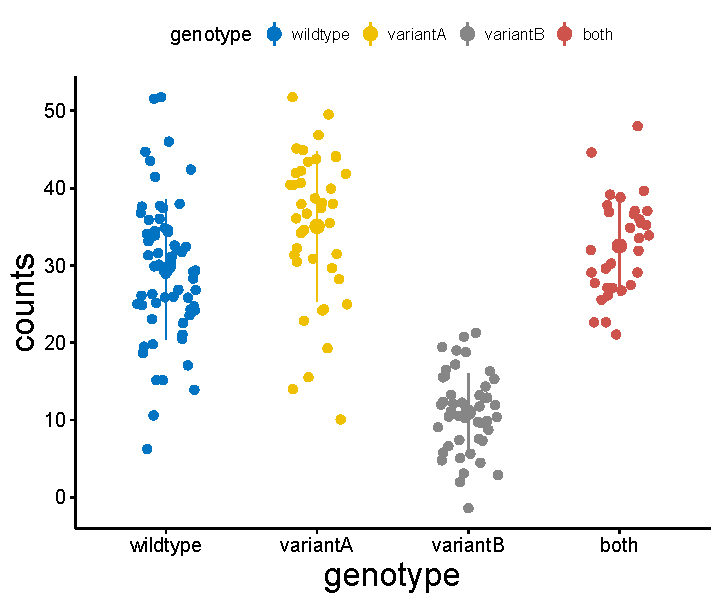
\includegraphics[width=0.8\columnwidth]{./Figures/genetic_interaction_concept.pdf}
	\caption{\textbf{Genetic interaction on transcriptome level:} Counts (expression) of a certain gene depend on the sample's genotype. In variant A the gene is similar expressed as in wildtype samples, whereas variant B clearly inhibits expression. If both variants co-occur this inhibition is reversed. Variant A either blocks the inhibitory effect of variant B or restores the expression by activation of an alternative pathway. By simple combination of the individual effects we would expect a phenotype similar to the one in variant B, thus both variants interact.}
	\label{fig:geneticInteraction}
\end{figure}

\FloatBarrier

\subsection{Gene expression in CLL}
The main challenge of gene expression profiling in CLL is the high heterogeneity. Many different clinical phenotypes varying in tumor progression and prognosis have been described. At the same time a high and growing number of genetic alterations in different combinations are found \citep{Landau2015}. This variety is also reflected on gene expression level and is one reason why only a few distinct associations between gene expression and CLL genotypes have been discovered so far. As consequence, a previous study with 121 CLL patients by \citet{Ecker2015} used gene expression variability instead of actual gene expression level to identify differentially regulated genes. Another study by \citet{Ferreira2014} identified two new subgroups based on transcriptome profiles in 98 CLL patients with stronger signatures than genotype associations. A later study associated these signatures with a technical blood sample processing signature, revealing technical noise as another bottleneck of transcriptome analysis in CLL \citep{Dvinge2014}. The PACE dataset contains the largest transcriptomic profiling dataset for CLL so far and also includes a variety of multi-omics datasets as well as clinical annotations, which provides us a powerful tool to further examine previous hypothesis and gain novel insights on the complex networks among genomic variation, transcription and phenotypes.










